%%%%%%%%%%%%%%%%%%%%%%% file template.tex %%%%%%%%%%%%%%%%%%%%%%%%%
%
% This is a general template file for the LaTeX package SVJour3
% for Springer journals.          Springer Heidelberg 2010/09/16
%
% Copy it to a new file with a new name and use it as the basis
% for your article. Delete % signs as needed.
%
% This template includes a few options for different layouts and
% content for various journals. Please consult a previous issue of
% your journal as needed.
%
%%%%%%%%%%%%%%%%%%%%%%%%%%%%%%%%%%%%%%%%%%%%%%%%%%%%%%%%%%%%%%%%%%%
%
% First comes an example EPS file -- just ignore it and
% proceed on the \documentclass line
% your LaTeX will extract the file if required
\begin{filecontents*}{example.eps}
%!PS-Adobe-3.0 EPSF-3.0
%%BoundingBox: 19 19 221 221
%%CreationDate: Mon Sep 29 1997
%%Creator: programmed by hand (JK)
%%EndComments
gsave
newpath
  20 20 moveto
  20 220 lineto
  220 220 lineto
  220 20 lineto
closepath
2 setlinewidth
gsave
  .4 setgray fill
grestore
stroke
grestore
\end{filecontents*}
%
\RequirePackage{fix-cm}
%
%\documentclass{svjour3}                     % onecolumn (standard format)
%\documentclass[smallcondensed]{svjour3}     % onecolumn (ditto)
\documentclass[smallextended]{svjour3}       % onecolumn (second format)
%\documentclass[twocolumn]{svjour3}          % twocolumn
%
\smartqed  % flush right qed marks, e.g. at end of proof
%
%
% \usepackage{mathptmx}      % use Times fonts if available on your TeX system
%
% insert here the call for the packages your document requires
%\usepackage{latexsym}
\usepackage{longtable}
\usepackage{xfrac}
\usepackage{graphicx}
% etc.
%
% please place your own definitions here and don't use \def but
% \newcommand{}{}
%
% Insert the name of "your journal" with
% \journalname{Molecular Breeding}
%
\begin{document}

\title{Developing a parsimonius predictor for binary traits in sugar
  beet (\emph{Beta vulgaris}) \thanks{Filippo Biscarini and Nelson Nazzicari contributed
    equally to the work.}
}
%\subtitle{Do you have a subtitle?\\ If so, write it here}

\titlerunning{Parsimonious predictor for binary traits in sugar beet}        % if too long for running head

\author{Filson Nazzarini         \and
        Simone Marini \and
	Piergiorgio Stevanato \and
	Nelppo Biscicari %etc.
}

%\authorrunning{Short form of author list} % if too long for running head

\institute{F. Biscarini, N. Nazzicari \at
              Fondazione Parco Tecnologico Padano \\
              %Tel.: +123-45-678910\\
              \email{filippo.biscarini@tecnoparco.org}           %  \\
%             \emph{Present address:} of F. Author  %  if needed
 \and
 S. Marini \at
    Dipartimento di Ingegneria Industriale e dell'Informazione \\
    Universit\`{a} di Pavia
\and
    P. Stevanato \at
    DAFNE, Universit\`{a} di Padova \\
    24105 Padova, Italy
}


\date{Received: 05 August 2014 / Accepted:}
% The correct dates will be entered by the editor

\maketitle

\begin{abstract}
Insert your abstract here. Include keywords, PACS and mathematical
subject classification numbers as needed.
\keywords{binary traits \and genomic predictions \and parsimonious predictor \and sugar beet}
% \PACS{PACS code1 \and PACS code2 \and more}
% \subclass{MSC code1 \and MSC code2 \and more}
\end{abstract}

\section{Introduction}
\label{intro}
The primary goal of breeding schemes in farm animals and crops is
generally to increase the agricultural output. Production traits are
typically quantitative continuous variables (e.g. milk
yield in dairy cattle, or per hectare yield in maize and rice).
Many traits of importance in plant and animal breeding follow nonetheless
a discrete categorical distribution, both ordered (e.g. calving ease in
cattle, grain texture in rice) and unordered
(e.g. grain pigmentation in rice, coat colour in cattle). A special case
is that of binomial traits, which can take up only two different values,
like disease resistance/susceptibility or presence/absence of a
morphological characteristic. 
Annual bolting (flowering) behaviour and root vigor are examples of binomial traits of agronomic
importance in sugar beet (\emph{Beta vulgaris}). [move this?] 

Advances in biotechnology and genomics, and the advent of high-density
molecular markers (especially sinlge-nucleotide polymorphisms, SNP)
genotyping have led to the emergence of molecular breeding
\cite{moose2008molecular}.
One exciting application of molecular breeding is genomic selection: the possibility of predicting the genetic value and future
performance of selection candidates solely from their genotypes (\cite{meuwissen2001prediction}). The predictive equations are
trained on reference individuals with both genotypic and phenotypic data and then
applied to selection candidates with genotypes only. Genomic selection
may bring about multiple benefits in breeding programmes such as
shorter breeding cycles or more efficient (e.g. traits difficult or
expensive to phenotype) and more accurate (e.g. traits with low
heritability) estimation of breeding values/selection
(\cite{goddard2007genomic,heffner2010plant}).
Key to the application of genomic selection to breeding programmes are reliable genomic
predictions.
The recent publication of the reference genome for \emph{Beta
vulgaris} genome \cite{dohm2013genome} is facilitating the application
of molecular breeding also in this crop species. Pioneering studies on
genomic predictions for both continuous (\cite{hofheinz2012genome,wurschum2013genomic}) and binary
(\cite{biscarini2014genome}) traits in sugar beet have already been published.

Genomic predictions are being based on increasing number of molecular
markers (e.g. 777K SNP-chip in cattle, 56K SNP-chip in maize,
whole-genome sequence data). When a huge number of potential predictors
is available, it may be useful to select a subset to limit laboratory
and bioinformatics costs, and the time of analysis, while at the same
time improving interpretability of results. There is therefore interest
in finding the minimum necessary set of information for a specific
problem. The principle of parsimony states that
a model needs to be simpler than the data the it explains (think for
instance of K-nearest neighbors -KNN- classifier with k=1), and according to Occam's razor, given two models that explain the data
equally well, the simplest has to be chosen (\cite{chaitin2006limits}).

The objective of this paper is to present the development of a
parsimonious predictor for the binary trait root vigor in a population
of sugar beet accessions.
SNPs in the panel were ranked based on their relevance and used to classify observations: one SNP at a
time was removed, progressively reducing the number of SNPs in the
predictive model.
We found that it was possible to strongly reduce the dimension of the
predictor and still achieve high accuracy.


\section{Material and methods}

\subsection{Plant material and SNP genotypes}
\label{sec:data}
The available population comprised 123 individual sugar beet (\emph{B. vulgaris})
plants, 100 with high- and 24 with low-root vigor. Root vigor is related
to nutrient uptake from the soil and plant productivity
(\cite{stevanato2010root}) and is recorded as a binary trait (either
high or low) based on the root elongation
rate of eleven-days-old seedlings. No predetermined root
elongation rate threshold was used to classify sugar beets into high or low
root vigour. The classification was subjectively made upon phenotypic
inspection and has nevertheless been shown to be robust over time (\cite{stevanato2010root}). 
The plant material was provided by Lion Seeds Ltd. (UK).

All plants were genotyped for 192 SNP markers with the
high-throughput marker array QuantStudio 12K Flex system
coupled with Taqman OpenArray technology. Additional details on the
genotyping procedure are described in Stevanato et al., 2013 (\cite{stevanato2013high}).
% There were in total 738  missing
% genotypes ($3.14\%$). Missing genotypes were imputed based on
% linkage disequilibrium (LD, \cite{browning2007rapid}).
After imputation and editing (call-rate $\geq 95\%$, MAF $\leq 2.5\%$)
175 SNPs were left for the analysis. A more detailed description of SNP
genotypes and editing procedure can be found in Biscarini et al. (\cite{biscarini2014genome}).
% Table~\ref{tab:overview}. Table~\ref{tab:chromosome} reports the
% distribution of the 175 SNPs (and related scaffolds) used in the
% analysis along the 9 chromosomes of the \emph{Beta
%   vulgaris} genome. The average scaffold size was $1037$ kbps
% (range: $34.5$ - $4957$ kbps).

\subsection{Predictor development procedure}
\label{sec:overview}
A two-step approach was adopted for the construction of a parsimonious
predictor for root vigor in sugar beet.
First, the 175 SNP available for the analysis after data editing were ranked based on their
relevance for predicting the trait under study.
In the second step the set of predictors was progressively reduced by
removing the least useful predictors one at a time. At each iteration
logistic regression was used to classify observations with the given set
of SNPs. 
As many classification results as the number of SNPs (i.e. 175) were
therefore obtained.

\subsubsection{Rank of predictors}
\label{par:boss}
When many predictors are availble -especially if $p>n$- it may be
of interest to reduce the dimensionality of the problem by choosing the
optimal subset of predictors that best describe the relationship between
dependent and independent variables [or that best model the response
variable, or are most informative with respect to the outcome to be
predicted, etc ...].
A Bayesian model selection method, the binary outcome stochastic search
(BOSS) algorithm \cite{russu2012stochastic}, was applied to identify the best set of predictive
SNPs by repeated sampling in a Markov Chain Monte
Carlo (MCMC) approach.  
SNPs were ranked based on their probability of inclusion in the best
predictive model.
 
In BOSS the relationship between binary observations and predictors is
described by a Gaussian latent variable model with a probit link function:

\begin{equation}
P(Y=[0/1]|X)=\phi(X \beta)
\label{eq:probit}
\end{equation} 

where $P(Y=[0/1]|X)$ is the probability of having low or high root vigor
given the SNP genotyps $X$, $\beta$ is a vector of regression
coefficients, and $\phi$ is the normal cumulative distribution function. 

The $n$ independent latent variables were normally distributed as $Z_i \sim
N(X_i^T\beta,1)$ (with $i=1 \ldots n$), and used to model the relationships between SNP genotypes and root vigor:

\begin{equation}
Y_i = \left\{ 
\begin{array}{ll}
0 \quad Z_i \leq 0 \\
1 \quad Z_i > 0
\end{array}
\right.
\quad \mathbf{Z}=\mathbf{X\beta+\epsilon}
\label{eq:threshold}
\end{equation}

% Prior distributions assigned
% to regression coefficients and model size, to specify prior belief on
% model complexity.
% Metropolis-Hastings sampling algorithm (check the Theory that would not die). 
BOSS extensively explores the model space to identify relevant
predictors, similar to what is done in Best Subset Selection (\cite{hastie2009model}).

%$\beta$ is assigned a multivariate Gaussian prior.

The selection of predictors was performed by introducing a vector of
indicator variables $\gamma=(\gamma_1, \ldots, \gamma_p)$ such that
$\gamma_i=0$ if $\beta_i=0$ and $\gamma_i=1$ if $\beta_i \neq 0$. A predictor
was included in the model if its regression coefficient was
not null and the associated indicator variable $\gamma=1$.
The model space to be searched was therefore given by the $2^p$ possible
combinations of SNPs (either included or excluded). This yielded a vector
$\beta_{\gamma}$ of size $p_{\gamma}$ with only the coefficients for which $\gamma_i=1$.

The prior for vector $\gamma$ was chosen from the following
beta-binomial (B) distribution: 

\begin{equation}
f(\gamma)=\frac{B(p_{\gamma}+a,p-p_{\gamma}+b)}{B(a,b)}
\label{eq:gammaprior}
\end{equation}

% \begin{equation}
% f(\mathbf{Z} | \gamma) = \int f(\mathbf{Z}|\gamma,\alpha,\beta_{\gamma})
% \end{equation}

with parameters $a$ and $b$ related to model size $p_{\gamma}$.

Knowing that the posterior conditional density for $\gamma$ is
proportional to its prior and the marginal likelihood of $\mathbf{Z}$,
the following holds: 

\begin{equation}
f(\gamma|\mathbf{Z}) \propto f(\gamma) \cdot f(\mathbf{Z}|\gamma)
\label{eq:gammapost}
\end{equation}

from which vector $\gamma$ can be sampled.
 
% Equation~\ref{eq:threshold} can be re-written as
% $\mathbf{Z=\alpha1+X_{\gamma}\beta_{\gamma}+\epsilon}$ and includes only
% predictors for which $\gamma=1$ ($\alpha$ is the intercept).


% $\gamma$ obtained through Binary Outcome Stochastic Search (BOSS): a
% sampling scheme from $f(\gamma|Z)$.

% Posteriors for $\beta$ through Gibbs sampling (again, see the Theory
% that would not die).

The BOSS algorithm is summarised below:

\begin{enumerate}
\item initialize the latent variables $\mathbf{Z}$;
\item sample $\gamma$ through a Metropolis-Hastings sampler (check the
  Theory that would not die) from its conditional posterior distribution
  in equation~\ref{eq:gammapost};
\item given $\mathbf{Z}$ and $\gamma$, sample $\beta_{\gamma}$ through
  standard Bayesian linear regression ($\mathbf{Z}=\mathbf{X_{\gamma}}\beta_{\gamma}+\epsilon$);
\item given $\beta_{\gamma}$ and $\mathbf{Y}$, sample the vector of latent
  variables $\mathbf{Z}$ from equation~\ref{eq:threshold};
\item restart from step 2 until $m=1\,000\,000$ iterations are completed
\end{enumerate}

From the $m=1\,000\,000$ MCMC iterations the inclusion probabilities for
the 175 SNPs were computed and used to rank the predictors.
A more detailed description of the BOSS algorithm can be found in Russu
et al. (\cite{russu2012stochastic}).

% The first step in our approach is to rank the SNPs by their informativeness
% on the studied phenotype trait. To do so we used one of the outputs of
% the BOSS algorithm \cite{russu2012stochastic}. This algorithm is designed
% to target binary traits, and performs a 
% a model search by sampling the predictors on the
% basis of a general and efficient Markov Chain
% Monte Carlo (MCMC) technique that exploits the
% conjugacy structure of data and parameters.

% The relationship between the observed
% responses and the available predictors is described
% by a latent variable model with a probit link. Prior 
% distributions are assigned both to
% the regression coefficients and the model size,
% therefore allowing the user to specify a prior
% belief on the model complexity. 

\subsubsection{Selection of predictors and classification method}
\label{par:predictor_selection}

SNPs were selected based on the BOSS rank (see section~\ref{par:boss})
by progressively removing one SNP at a time. The full set of 175 SNPs
was used at first in the prediction model. Subsequently, the $m^{th}$ least
relevant SNP (from the BOSS rank) was removed each time, and the
resulting $175-m$ SNPs model was fitted. As a result of this, 175
different predictive models (from 175 to 1 predictor) were fitted.

With each set of SNP, a logistic regression model for binary outcomes
was used to classify observations into low and high root vigor based on
the SNP genotypes. The probability having high root vigor ($P(Y=1|X)=p(x)$) was modeled as a linear
combination of the predictors (SNPs) through a \emph{logit}
link-function in a generalised linear model:

\begin{equation} \label{eq:logistic}
logit(p(x_i)) = log \left ( \frac{p(x_i)}{1-p(x_i)} \right ) = \mu +
\sum_{j=1}^m z_{ij} SNP_j
\end{equation}
 
where $p(x_i)$ is the $P(Y=1|X)$ for individual $i$ with vector of
predictors $x_i$; $SNP_j$ is the effect of the $j_{th}$ marker; $z_{ij}$
is the genotype of individual $i$ at locus $j$ (0, 1 or 2 for AA, AB and
BB genotypes).
Equation~\ref{eq:logistic} returns the odds of $p(x)$ which are
backtransformed to $P(Y=1|X)$ through the cumulative
distribution function of the logistic distribution (i.e. the logistic
function). Individuals with $p(x)>/<0.5$ were classified as high/low
root vigor individual plants.

Since there were more predictors than observations in
model~\ref{eq:logistic} ($p>n$), a ridge logistic regression fitting method
\cite{liu2011multilocus} was adopted, which consisted in maximizing the following
penalized log-likelihood:

\begin{equation}
L(\mu,SNP)=\sum_{i=1}^n
[y_ilog(p_i)+(1-y_i)log(1-p_i)]-\frac{1}{2}\lambda\sum_{j=1}^p SNP_j^2
\end{equation}

where $\mu$ is the intercept, $SNP$ is the vector of SNP effects (i.e. the
regression coefficients of SNP genotypes) and $\lambda$ is a tuning
parameter that was specified through cross-validation and controls the
amount of penalization.

\subsubsection{Predictive ability}
\label{par:estimating_error}
For each set of SNPs (175 to 1), the predictive ability of
the ridge logistic regression model (equation~\ref{eq:logistic}) was assessed
through a two-fold cross-validation. 
The 123 samples were randomly split into a training and testing set of approximately equal
size. The training set was used to fit the model and estimate SNP
effects which were then used to predict root vigor in the testing set. This process was repeated 100
times, each time sampling different training and testing sets.  
The test error rate in each replicate was computed as:

\begin{equation} \label{eq:testerr}
 ER_{(n)}=\frac{1}{n} \sum_{i=1}^{n} Err_i
\end{equation}

where $n$ is the number of observations in the test set and $Err_i=I(y_i \neq \hat{y}_i)$, with $I(\cdot)$ an indicator function
which returns a value of 1 if the predicted and observed phenotypes are
different, 0 otherwise. 
The cross-validation error rate was then estimated averaging the test error
rate over all $k=100$ replicates:

\begin{equation} \label{eq:cverr}
CV_{k}=\frac{1}{k} \sum_{i=1}^k ER_i
\end{equation}

The prediction accuracy was then defined as $1-CV_k$. Besides the total
error rate, also the false positive (FPR) and false negative (FNR) rates
were computed. False positives (FP) were defined as true low-root vigor
plants predicted as high-root vigor, whereas false negatives (FN) were
defined as true low-root vigor plants predicted as high-root vigor.
Then, $FPR=\sfrac{FP}{N}$ and $FNR=\sfrac{FN}{P}$, where $N$ and $P$ are
the total number of true negative (low-root vigor) and true positive
(high-root vigor) samples.

\subsection{Comparison with another method to rank predictors}
\label{sec:other_ranker}
The BOSS algorithm yielded a rank of the SNPs based on their probability
of inclusion in the best predictive model. SNPs could be ranked also
based on different metrics. For instance, the relative effect on the
trait under analysis could be chosen as an indirect measure of the
predictive importance of the SNPs.

A logistic model of the form $logit(p_i)=\mu+SNP_m$ ($i=1,\ldots,123$
plants; $m=1,\ldots, 175$ SNPs) was fit one SNP
at a time in order to estimate marker effects.
From estimated marker effects and allele frequencies, the additive
genetic variance at each SNP locus was estimated as:

\begin{equation}
V_A=2pqa^2
\end{equation}

where $p$ and $q$ are the frequencies of the two alleles in the
population and $a$ is the marker additive effect
(\cite{gianola2009additive}).
SNPs were then ranked based on decreasing genetic variance and used for
predictor selection and classification as in
section~\ref{par:predictor_selection}. Prediction accuracy was estimated
as in section~\ref{par:estimating_error}.

\subsection{Software}
\label{sec:software}
\emph{Matlab} scripts \cite{MATLAB2010} were used to implement the BOSS
algorithm for model selection. Classification of observations was done
with the Java data mining software \emph{Weka 3} \cite{hall2009weka}.
The open source statistical environment \emph{R} \cite{r2008manual} and
the open source spreadsheet \emph{Gnumeric 1.12.12}
(\cite{gnumeric2014}) were used for data manipulation, the creation of
figures and all other statistical analyses.

\section{Results}
\label{sec:results}
Supplementary table with BOSS rank of SNPs (Table~\ref{tab:rank}: use
SNP name instead of order, add scaffold and chromosome). A few comments on the most
important SNPs (which ones, on which chromosomes, how many per
chromosome ...).

Figure~\ref{fig:accuracy}: Accuracy as a function of the number of
predictors, BOSS vs logistic [improve plot: no need to go down to 0.0 in
the y-axis; legend names and position; color of the lines? The ``bump''
at around 20-30 SNPs is not visible]

Table~\ref{tab:error}: TER, FPR, FNR for the first 30/35 SNPs + average for the
rest of the SNP (error close to $0$). BOSS + GWAS (6 columns)


Probability of assignment as a function of predictors:
Figure~\ref{fig:probability}. Better a table? Maybe in discussion?

From ROC curves only the AUC. No plot, use AUC as result in the text (e.g.
comparison between ranker: overall average AUC, average AUC per \# SNPs
+ std). Table?

% For one-column wide figures use
\begin{figure}
% Use the relevant command to insert your figure file.
% For example, with the graphicx package use
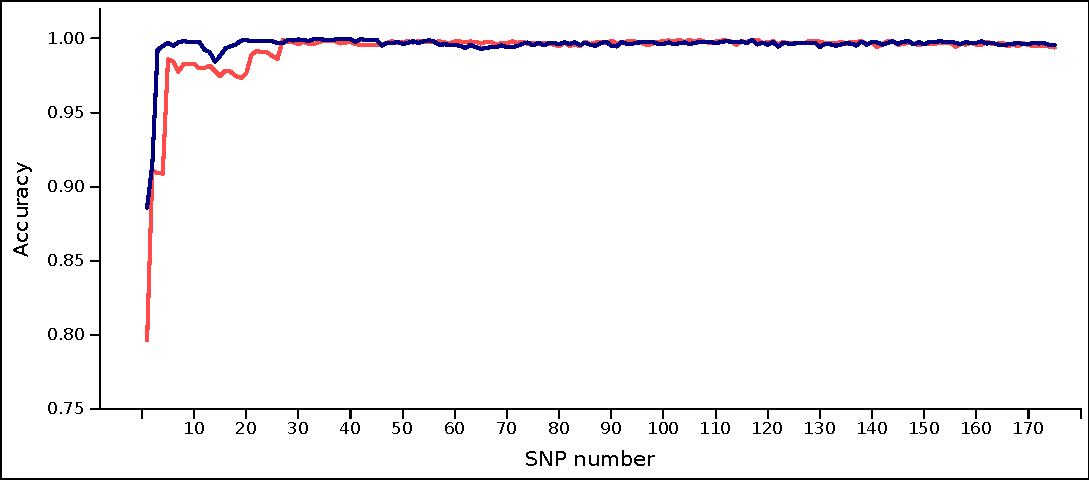
\includegraphics[width=0.95\textwidth]{accuracy.pdf}
% figure caption is below the figure
\caption{Accuracy (1 - error rate) of prediction as a function of the
  number of SNPs included in the classifier: BOSS (blue line) vs
  logistic regression (red line)}
\label{fig:accuracy}       % Give a unique label
\end{figure}

\begin{figure}
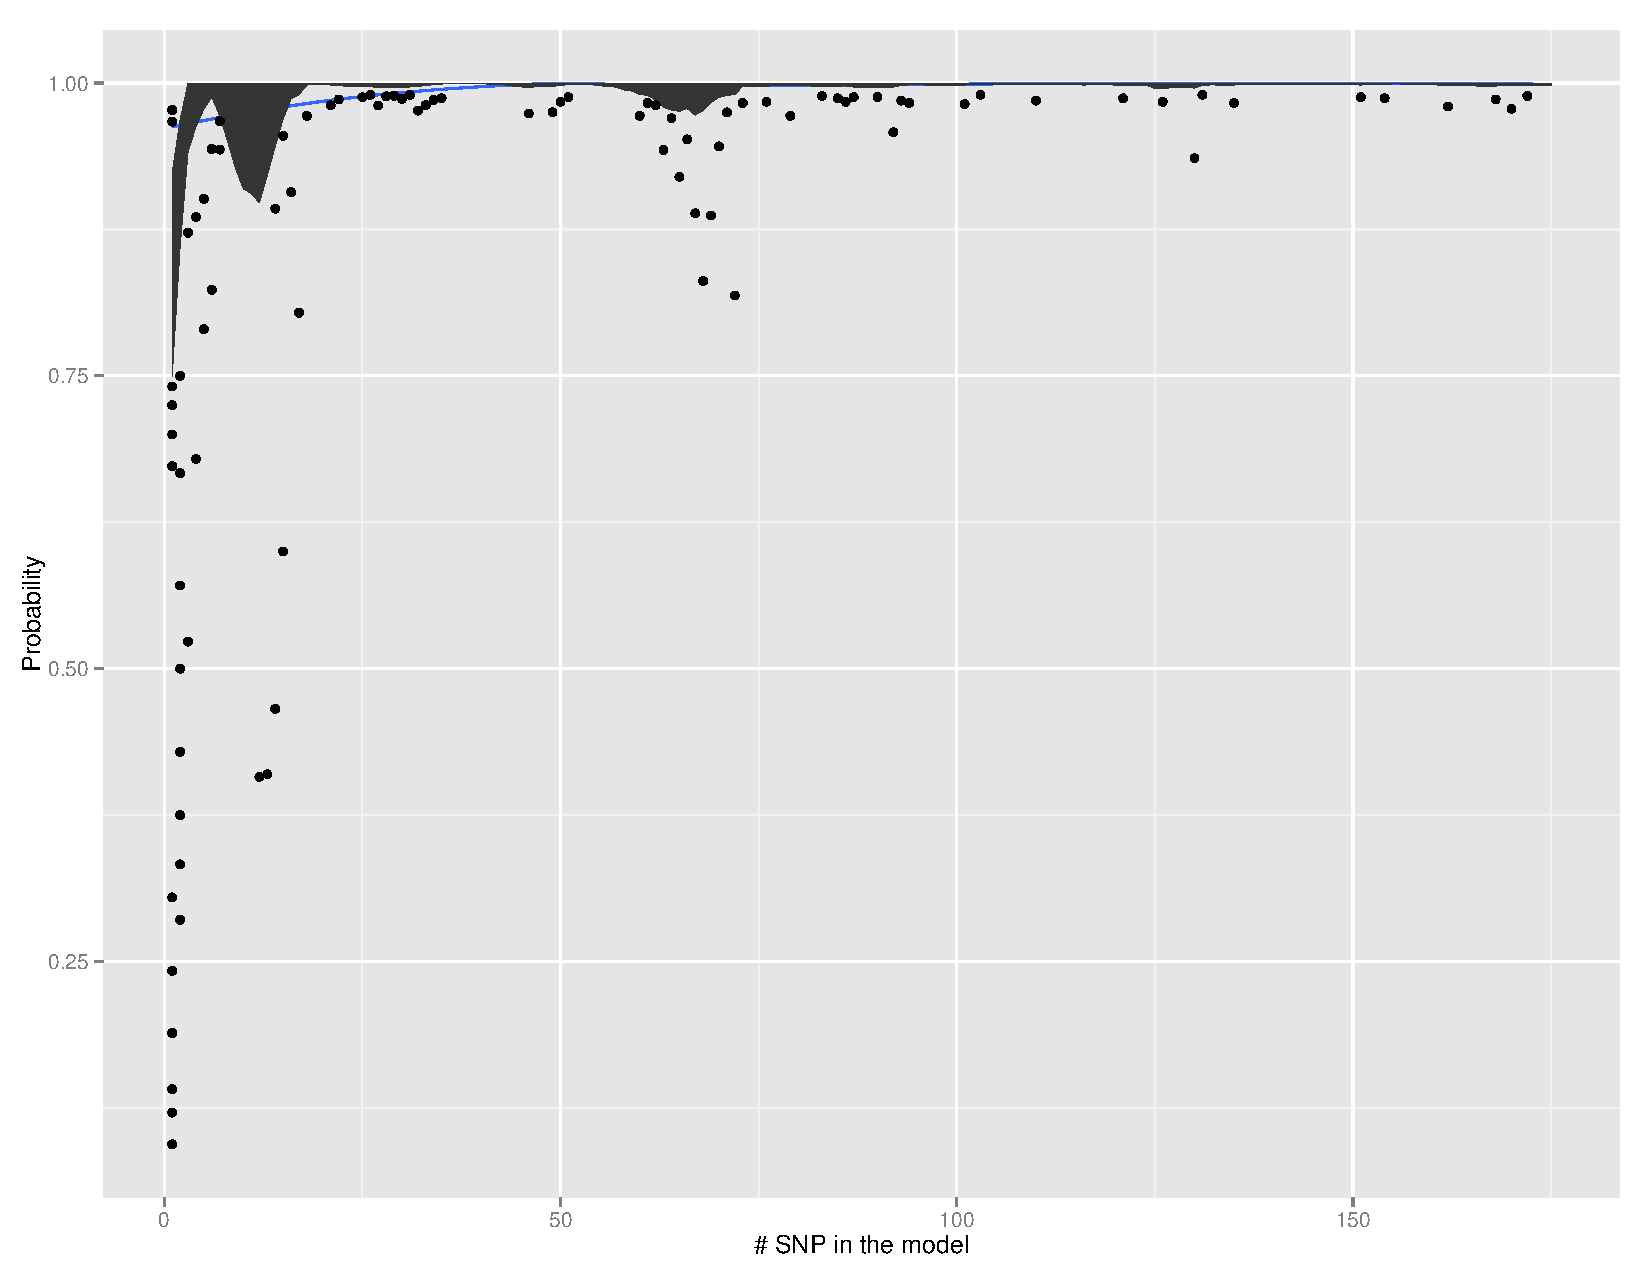
\includegraphics[width=0.95\textwidth]{probabilities.pdf}
\caption{Distribution of $P(Y=1|x)$ as a function of the number of SNPs
  in the classifier}
\label{fig:probability} 
\end{figure}


\section{Discussion}
\label{sec:discussion}
General overview
why error rates are not evenly distributed?
Reminder: it works very well because of LD and H2

Unstable below 30/40 SNPs; little ``bump'' around 20 SNPs: more marked
with BOSS, but also visible with GWAS. Why there? SNPs with large effect
on the trait, but low significance? SNPs with large effect but low LD
(with the QTL)? In the latter case, the marker might sometimes be in the
opposite phase. Look also at marker frequency.

Based on results, a panel of 30-35-40 SNPs is recommended for accurate
prediction of root vigor (move to breeding applications? Together with
development of a custom-chip?)

\begin{figure}
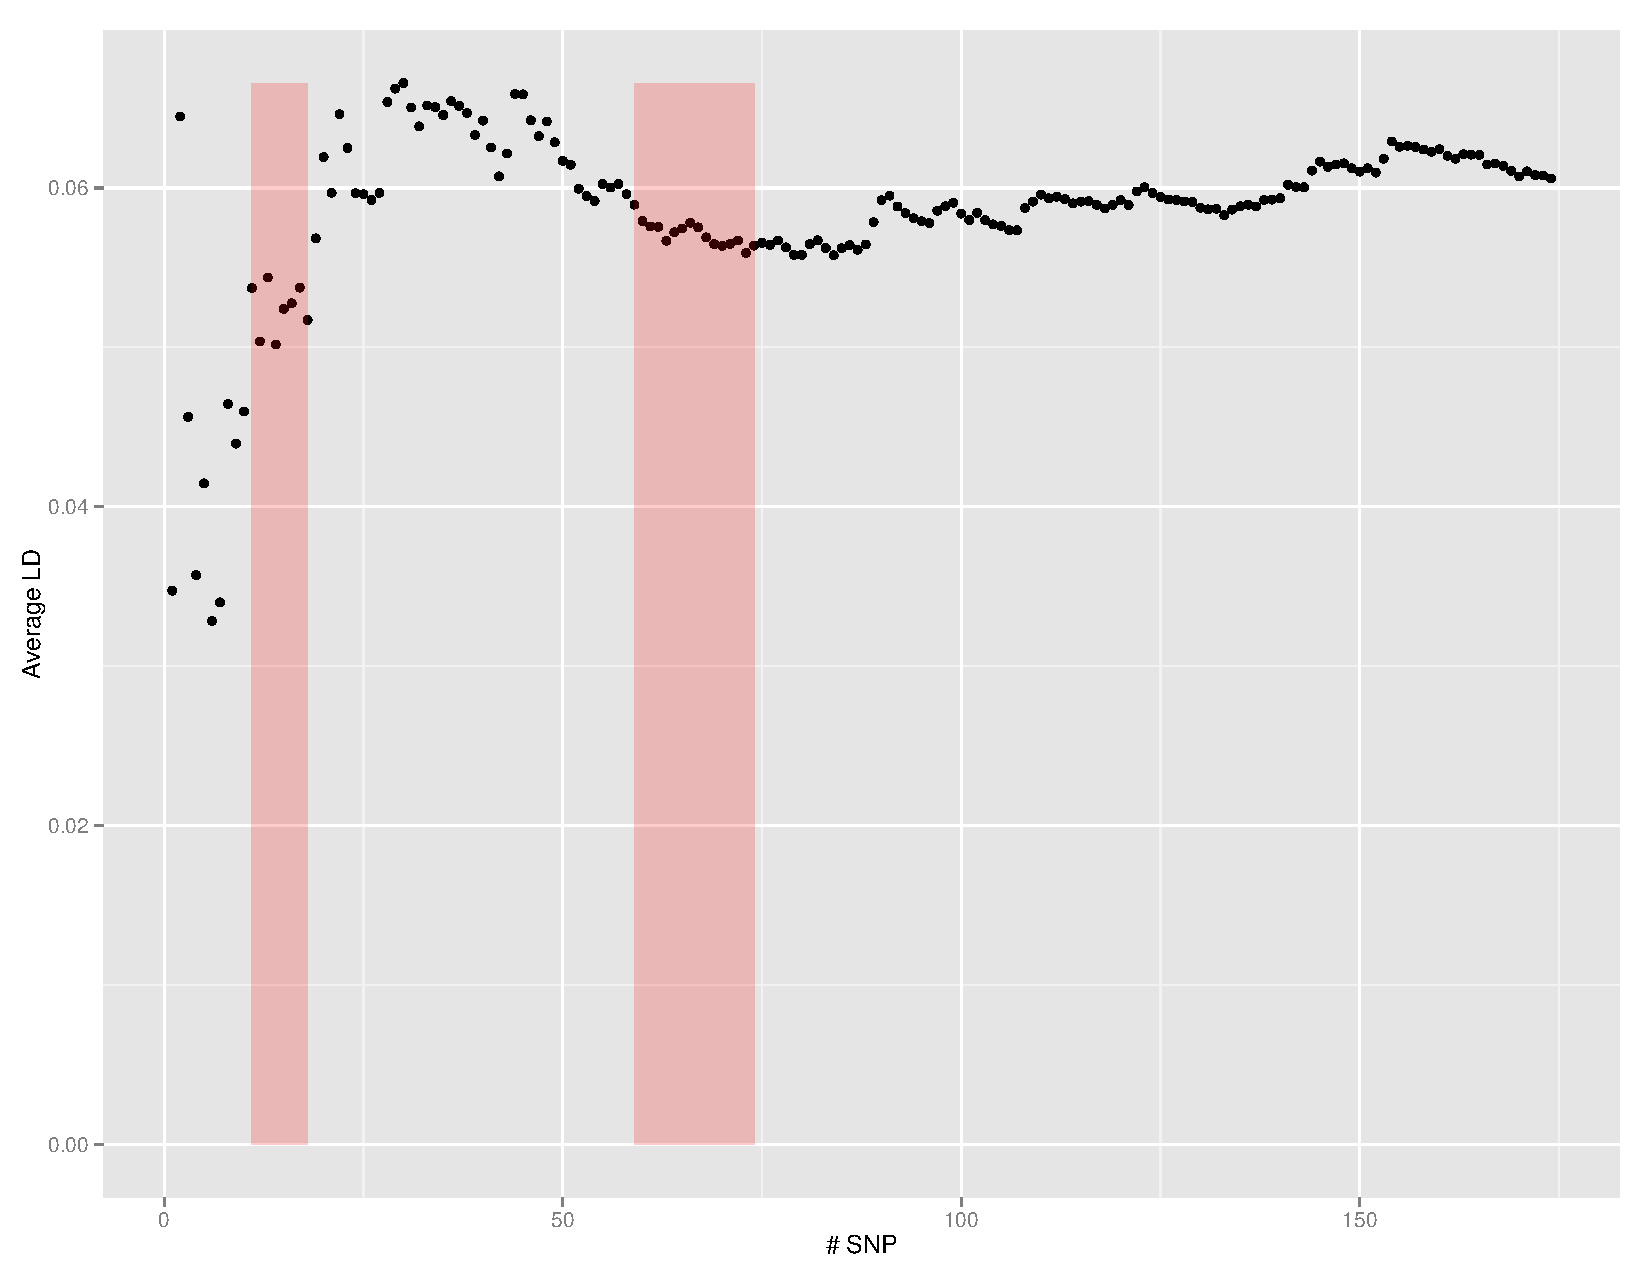
\includegraphics[width=0.95\textwidth]{LD.pdf}
\caption{Average linkage disequilibrium (LD) for increasing number of
  SNPs in thepredictive model}
\label{fig:ld} 
\end{figure}

\subsection{Relative performance of rankers}
why using Pvalues and not other standard rankers (e.g. backward stepwise
selection)? Because of the specific nature of the problem. ROC and AUC?

Comparison of rankers: spearman correlation + plot (ranker1 vs ranker2).

Figure~\ref{fig:rank}

\begin{figure}
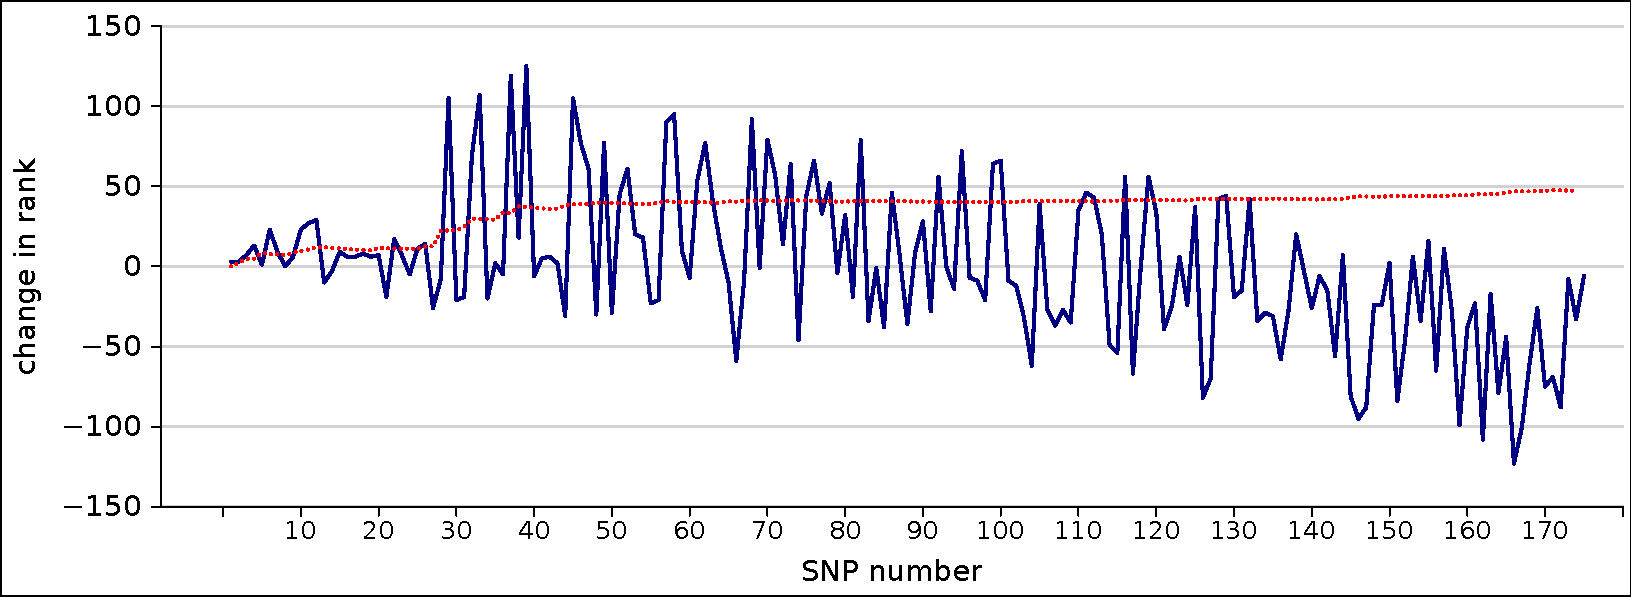
\includegraphics[width=0.95\textwidth]{rank.pdf}
\caption{Comparison of BOSS and logistic regression in terms of relative
rank position of relevant SNPs}
\label{fig:rank} 
\end{figure}


\subsection{SNP effects [alternative: LD and probabilities]}
Manhattan plot with BOSS weights and weights from the other articles,
somehow compared (same chart? two charts? only ten best?).

Let's not use effects from GWAS (the paper is on BOSS!!): something on
the top ranked SNPs (position ...)?

Do the peaks make sense from the biological perspective? (something on
sugar beet genes?)

Variance of SNPs vs genetic variance: $\rightarrow$ missing
heritability? (cite Brachi 2011, Manolio 2009?).

BOSS probability: 1 big peak + smaller peaks. Compare against SNP
density? Maybe the big peak corresponds to a physically isolated SNP,
whereas smaller peaks correspond to a cluster of SNPs in LD which
individually account for a smaller part of the variatino, but together
play an important predictive role. 


\subsection{Genotyping strategies and applications to breeding}
Several techology choices are commonly available when genotyping strategies
must be decided. Assuming knowledge of SNP flanking sequences, we examine
four options: SNP chips, genotyping by sequencing (GBS), targeted sequencing (TS),
and a commercial solution, Illumina BeadXpress.


Genotyping by sequencing is 

genotyping strategies: 
Costs, possible technologies (gbs, snp chip, macroarrays), implications

applications to breeding:
why is it important root vigor early detection. Other binomial traits (e.g.
disease resistance) May be applied to bolting (another trait which
exhibits binomial distribution), which has been shown to be controlled
by multiple genes and influenced by environmental factors
(\cite{salah2012genetic}).

sugar beet: $30\%$ of world's sugar production (cite Dohm? FAO?). Root
vigor linked to yield.

Sugar beet: sugar + energy (citation?)

Other binomial traits: resistance to viral and fungal diseases, bolting
(cite Dohm? Someone else?)

Breeding has shaped the genome of sugar beet (comparison with \emph{Beta
  maritima}, \cite{dohm2013genome}).

Extensions to multinomial traits? Examples?

potential and challenges of genomic selection in plant breeding (\cite{jonas2013does})

% For two-column wide figures use
%\begin{figure*}
% Use the relevant command to insert your figure file.
% For example, with the graphicx package use
%  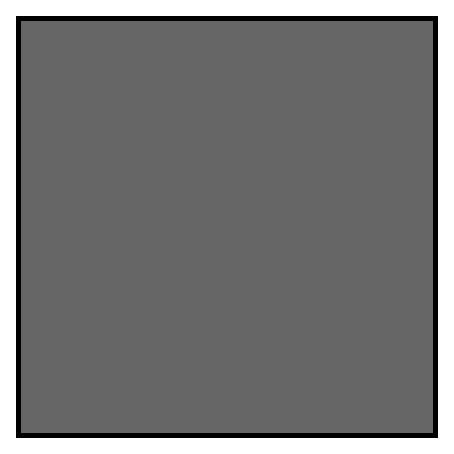
\includegraphics[width=0.75\textwidth]{example.eps}
% figure caption is below the figure
%\caption{Please write your figure caption here}
%\label{fig:2}       % Give a unique label
%\end{figure*}
%

\section{Conclusions}
\label{sec:conclusions}

Concluding remarks. 


\begin{acknowledgements}
This research was financially supported by the Marie Curie European
Reintegration Grant ``NEUTRADAPT''.
\end{acknowledgements}

%\section{Tables}

% For tables use
\begin{table}
\centering
% table caption is above the table
\caption{Total error rate (TER), false positive (FPR) and false negative
  (FNR) rates as a function of the number of SNPs incluided in the
  model, for both the BOSS and SNP variance rankings}
\label{tab:error}       % Give a unique label
% For LaTeX tables use
\begin{tabular}{ccccccc}
\hline\noalign{\smallskip}
 & \multicolumn{3}{c}{BOSS} & \multicolumn{3}{c}{SNP Variance}\\
\noalign{\smallskip}\hline\noalign{\smallskip}
\# SNPs & TER & FPR & FNR & TER & FPR & FNR\\
\noalign{\smallskip}\hline\noalign{\smallskip}
1 & 0.114 & 0.333 & 0.061 & 0.204 & 0.500 & 0.132\\
2 & 0.085 & 0.192 & 0.059 & 0.089 & 0.002 & 0.111\\
3 & 0.008 & 0.033 & 0.002 & 0.091 & 0.001 & 0.113\\
4 & 0.005 & 0.025 & 0.001 & 0.091 & 0.001 & 0.113\\
5 & 0.003 & 0.006 & 0.002 & 0.014 & 0.000 & 0.017\\
6 & 0.005 & 0.011 & 0.004 & 0.016 & 0.001 & 0.019\\
7 & 0.003 & 0.005 & 0.002 & 0.022 & 0.001 & 0.028\\
8 & 0.002 & 0.002 & 0.002 & 0.017 & 0.000 & 0.022\\
9 & 0.003 & 0.000 & 0.003 & 0.017 & 0.000 & 0.022\\
10 & 0.002 & 0.001 &  0.003 & 0.017 & 0.000 & 0.021\\
11 & 0.002 & 0.001 &  0.002 & 0.020 & 0.001 & 0.025\\
12 & 0.008 & 0.001 &  0.009 & 0.020 & 0.002 & 0.024\\
13 & 0.009 & 0.001 &  0.011 & 0.018 & 0.001 & 0.023\\
14 & 0.016 & 0.000 &  0.019 & 0.022 & 0.001 & 0.027\\
15 & 0.012 & 0.000 &  0.015 & 0.025 & 0.003 & 0.032\\
16 & 0.007 & 0.001 &  0.008 & 0.022 & 0.002 & 0.027\\
17 & 0.005 & 0.000 &  0.007 & 0.022 & 0.001 & 0.027\\
18 & 0.004 & 0.001 &  0.005 & 0.025 & 0.002 & 0.032\\
19 & 0.002 & 0.001 &  0.002 & 0.027 & 0.002 & 0.033\\
20 & 0.001 & 0.000 &  0.001 & 0.022 & 0.001 & 0.029\\
21--30 & 0.002 & 0.001 & 0.002 & 0.007 & 0.003 & 0.008\\
31--40 & 0.001 & 0.000 & 0.001 & 0.003 & 0.002 & 0.003\\
41--50 & 0.004 & 0.001 & 0.003 & 0.004 & 0.002 & 0.004\\
51--60 & 0.002 & 0.001 & 0.004 & 0.004 & 0.004 & 0.003\\
61--70 & 0.003 & 0.001 & 0.007 & 0.003 & 0.003 & 0.002\\
71--80 & 0.004 & 0.001 & 0.005 & 0.003 & 0.003 & 0.003\\
81--90 & 0.002 & 0.004 & 0.002 & 0.003 & 0.004 & 0.003\\
91--100 & 0.001 & 0.001 & 0.001 & 0.003 & 0.003 & 0.002\\
101--175 & 0.001 &  0.002 & 0.001 & 0.002 &  0.005 & 0.002\\
\noalign{\smallskip}\hline
\end{tabular}
\end{table}




% BibTeX users please use one of
%\bibliographystyle{spbasic}      % basic style, author-year citations
\bibliographystyle{spmpsci}      % mathematics and physical sciences
%\bibliographystyle{spphys}       % APS-like style for physics
\bibliography{parsimonious.bib}   % name your BibTeX data base

% Non-BibTeX users please use
%\begin{thebibliography}{}
%
% and use \bibitem to create references. Consult the Instructions
% for authors for reference list style.
%
%\bibitem{RefJ}
% Format for Journal Reference
%Author, Article title, Journal, Volume, page numbers (year)
% Format for books
%\bibitem{RefB}
%Author, Book title, page numbers. Publisher, place (year)
% etc
%\end{thebibliography}

\end{document}
% end of file template.tex

